\chapter{复合物筛选模型设计}
\label{chapter:gcnfilter}

\section{相关算法介绍}
\label{section:arithmetic}
\subsection{图卷积神经网络}
\label{subsection:GCN}
\subsection{网络嵌入}
\label{subsection:nodeEmbedding}
\subsection{图自编码器}
\label{subsection:GAE}
\section{算法总体流程}
\label{section:progress}

复合物筛选模型框架设计如图\ref{fig:main-process}所示;

\begin{figure}[htbp]
    \centering
    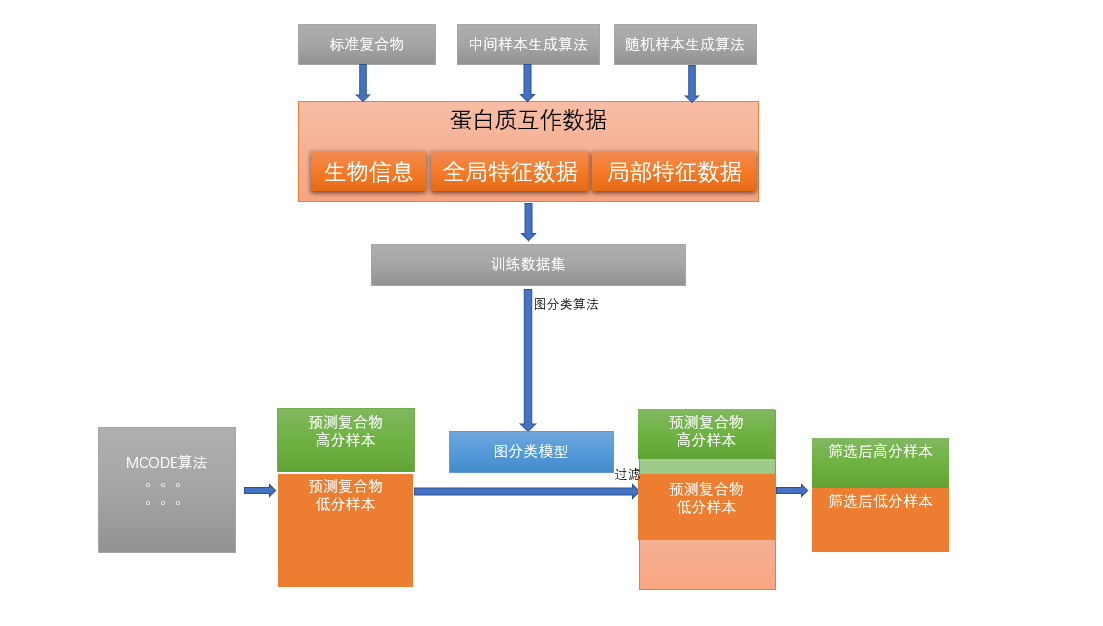
\includegraphics[width=14cm]{main-process}
    \caption{复合物筛选框架主体流程图}
    \label{fig:main-process}
\end{figure}

首先依照\ref{section:datasetExtract}提出的数据集构建方法,对每一个复合物网络可以得到一个由复合物子图构成的数据集。该数据集中每一个复合物子图有和标准复合物的邻居相似性评分,总体分为四类复合物,分别为标准复合物、高评分预测复合物、低评分预测复合物和随机复合物。

第一阶段,提出合适的复合物分类模型,并基于该数据集训练复合物分类模型\ref{section:GlobalfeatBaseModel}。

第二阶段,在蛋白质相互作用网络中得到复合物预测算法,如MCODE算法、clique算法等的预测结果。依据复合物分类结果的评价方法,在这些预测结果中,有一部分高分样本复合物预测符合预期结果,如图中绿色部分所示,其余部分为低分复合物样本,如图中红色部分所示。下一步利用复合物分类模型对所有的样本进行筛选,通过筛选的复合物符合模型学习到的复合物一般分布规律,筛选之后保留的复合物如图最终输出结果所示。

第三阶段,本文使用多种的复合物预测评价指标对筛选前后的总体样本进行综合评价。



\section{基于全局特征的模型}
\label{section:GlobalfeatBaseModel}

\subsection{模型提出}
\label{subsection:Global:Modelget}
已有的基于监督学习的复合物预测算法,基本都是基于挖掘复合物子图的拓扑特征,比如图的密度、图的结点个数、平均度数等等,将图的所有拓扑特征置于一个向量中,构成一个$1\times N$的向量,用该向量代替子图,最后将向量用于训练分类模型。具体过程如图\ref{fig:entropy-classification}所示。

\begin{figure}[htbp]
    \centering
    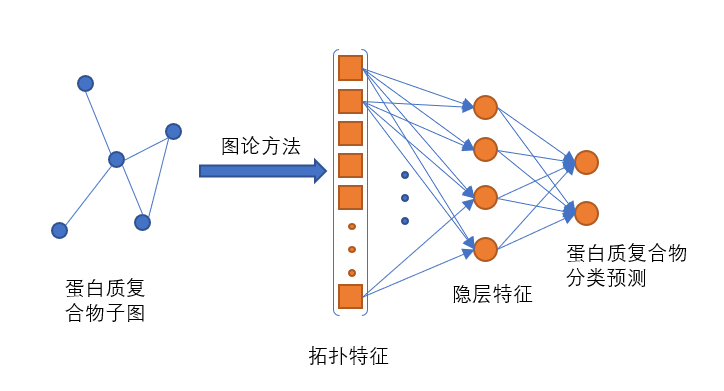
\includegraphics[width=14cm]{entropy-classification}
    \caption{基于图拓扑特征的蛋白质复合物分类模型}
    \label{fig:entropy-classification}
\end{figure}


但是蛋白质复合物中,有大部分复合物是小尺度复合物,其蛋白质个数小于5个。此类复合物的拓扑结构结构简单,提取的拓扑特征具有趋同性。随机的子图在结点数较少的情况下可能形成相同的拓扑特征,此时分类模型无法区分子图是否为真正的复合物。

为了解决该问题,在不引入额外的生物学信息的情况下,本文提出了基于全局特征的复合物分类模型。
蛋白质复合物网络是一个高维结构,可以通过挖掘蛋白质在网络中所处的位置和其周围相互作用关系挖掘蛋白质的潜在特征表示,将网络的高维数据转换为蛋白质的低维嵌入表示,成为每一个蛋白质初始的特征向量。

\subsection{模型细节}
\label{subsection:Global:Modeldetail}
本文使用了两种蛋白质特征嵌入模型,分别为Deepwalk和GAE。

Deepwalk基于蛋白质为源点在$PIN$网络中随机游走,得到随机游走序列,该序列为图中结点与结点共现关系的描述。通过Word2Vec的方式,获取序列中每一个结点的向量表示。本文得到的Deepwalk产生的结点特征维度为64维。

GAE基于蛋白质复合物网络的编码与解码实现。蛋白质分子的初始特征为随机特征,编码过程采用2层GCN网络,得到蛋白质分子的隐层表示,解码过程通过结点隐层表示预测结点之间的连接强度,恢复网络拓扑结构。损失函数为预测的$PIN$邻接矩阵和真实邻接矩阵的MSELoss(Mean Square Error Loss)。本文得到的GAE产生的结点特征维度为16维。
\subsection{模型流程}
\label{subsection:Global:Modelflow}
\begin{figure}[htbp]
    \centering
    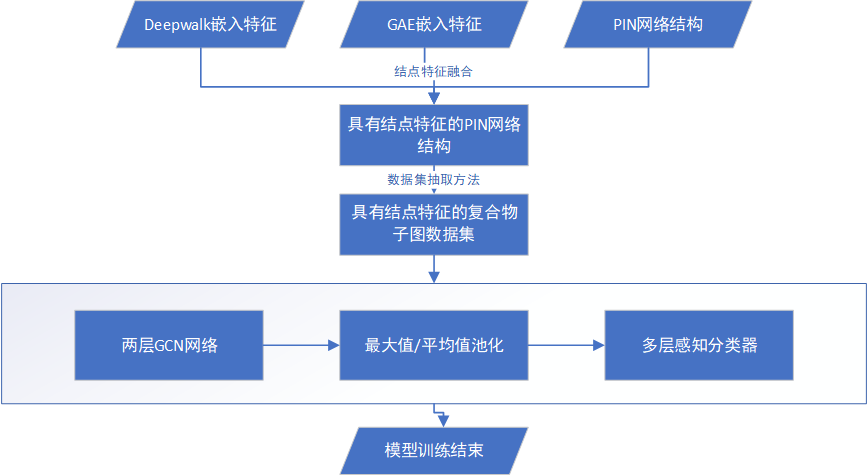
\includegraphics[width=14cm]{node-classification-flow}
    \caption{基于全局特征的分类模型总体流程}
    \label{fig:node-classification-flow}
\end{figure}
基于全局特征的复合物分类模型总体结构如图\ref{fig:node-classification-flow}所示。基于Deepwalk和GAE编码,蛋白质嵌入特征维度总共80维,在$PIN$中加入嵌入特征之后,蛋白质复合物子图具备了初始的结点特征向量。图卷积神经网络\ref{subsection:GCN}具有动态融合结点特征和拓扑结构的能力,已经广泛应用于图任务中。
初始嵌入的80维特征是整个$PIN$网络中结点特征的描述,但是还未结合蛋白质复合物子图的拓扑关系。因此,本文在后续的图分类任务中加上了两层GCN网络对蛋白质结点特征和子图拓扑结构进行融合,增加蛋白质结点特征对复合物内部蛋白质互作关系的描述能力。
最终基于全局特征的复合物分类模型对子图的蛋白质结点特征做平均池化,作为蛋白质复合物特征的输出,以多层感知器预测复合物的分类结果。


\section{基于生物特征的模型}
\label{section:biofeatBaseModel}
\subsection{模型提出}
\label{subsection:biofeat:Modelget}
已有方法已经充分表明,在PPI网络中进行蛋白质复合物预测不仅仅是一个图论中的聚簇发现问题,更是一个信息融合问题。无论是加权网络方法、核心附属结构预测方法,都致力于最大程度的利用生物学信息进行辅助预测。基于该前提,本文提出了基于生物特征的复合物预测模型。
\subsection{模型细节}
\label{subsection:biofeat:Modeldetail}
如表\ref{subsection:SimSummary}所示,本文处理了大量的生物学数据,包括蛋白质功能注释数据、结构域相互作用数据、亚细胞定位数据等,应用相关的生物邻域的处理方法将生物学数据转换为可应用的特征数据,最终得到了12维度的特征数据。所有的特征都描述蛋白质相互作用,因此在图结构中,这些特征编码为图结构邻边的特征。

如\ref{subsection:GCN}介绍,已有的图卷积方法为基于结点的卷积算法。在子图结构中,生物信息只能被映射为邻边信息,为了将邻边信息转换为结点信息,本文提出了从邻边到结点的信息汇聚过程。

在通常的图卷积过程中,结点A的特征为周围所有结点的特征和自生特征决定,可以采取平均值的计算方法,如公式\ref{equ:NormalGCNNodeFlow}所示。
\begin{equation}
    \label{equ:NormalGCNNodeFlow}
    f_a=\delta (\frac{\sum_{i = 1}^{n}f_i+f_a}{n+1})
\end{equation}
其中$f_a$代表A结点的特征,$f_i$代表A结点所有邻居的特征,$\delta$为信息汇聚之后的特征更新函数。
在汇聚结点周围邻边的特征计算方法中,结点特征由其邻边共同决定。其具体计算过程如公式\ref{equ:EdgetoNodeFeat}所示。
\begin{equation}
    \label{equ:EdgetoNodeFeat}
    f_a=\delta (\frac{\sum_{i = 1}^{n}f_{ia}}{n})
\end{equation}
其中$f_{ia}$表示所有连接到A的邻边特征。其具体的汇聚过程如图\ref{fig:edge-feat-flow}所示,A结点汇聚周围所有邻边特征,包括$F_{BA}$、$F_{CA}$、$F_{DA}$以及$F_{EA}$。

\begin{figure}[htbp]
    \centering
    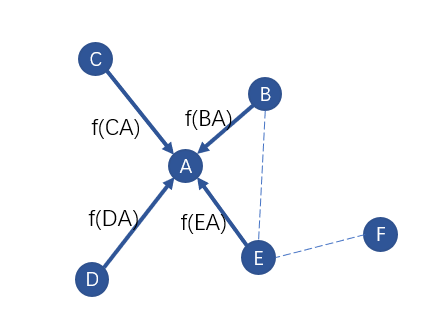
\includegraphics[width=7cm]{edge-feat-flow}
    \caption{边特征初始化结点特征示意图}
    \label{fig:edge-feat-flow}
\end{figure}

蛋白质生物数据是基于邻边的数据,因此在对复合物子图做图卷积的时候,基于生物特征的模型采用了基于edge的GCN模型\cite{wang_dynamic_2019},其具体的邻边更新方式如式\ref{equ:EdgeConv}所示。
\begin{equation}
    \label{equ:EdgeConv}
    h_i^{(l+1)} = \max_{j \in \mathcal{N}(i)} \mathrm{ReLU}(
    \Theta \cdot (h_j^{(l)} - h_i^{(l)}) + \Phi \cdot h_i^{(l)})
\end{equation}
其中$h_i^{(l+1)}$表示第$l+1$层更新之后的结点数据,$h_j^{(l)} - h_i^{(l)}$表示从邻居结点到$i$结点的数据流,$h_i^{(l)}$为结点保留信息,$\Theta$和$\Phi$分别对应更新函数。
\subsection{模型流程}
\label{subsection:biofeat:Modelflow}
首先将生物特征GO注释、拓扑域相似性、亚细胞定位特征整合到一起,嵌入到PPI网络的邻边作为邻边特征。再使用复合物子图抽取方法从网络中获取训练数据集,包括正样本、负样本和中间样本。
然后使用特征汇聚方法将邻边特征汇聚到结点特征中,再使用基于edge更新的图卷积方法进行特征融合。
本文在图分类任务中加上了两层基于邻边的图卷积网络对生物特征和子图拓扑结构进行融合。图读出阶段使用了基于结点的平均池化和最大值池化方法。最终的分类阶段使用了两层感知器模型。
基于生物特征的复合物分类模型总体结构如图\ref{fig:edge-classification-flow}所示。
\begin{figure}[htbp]
    \centering
    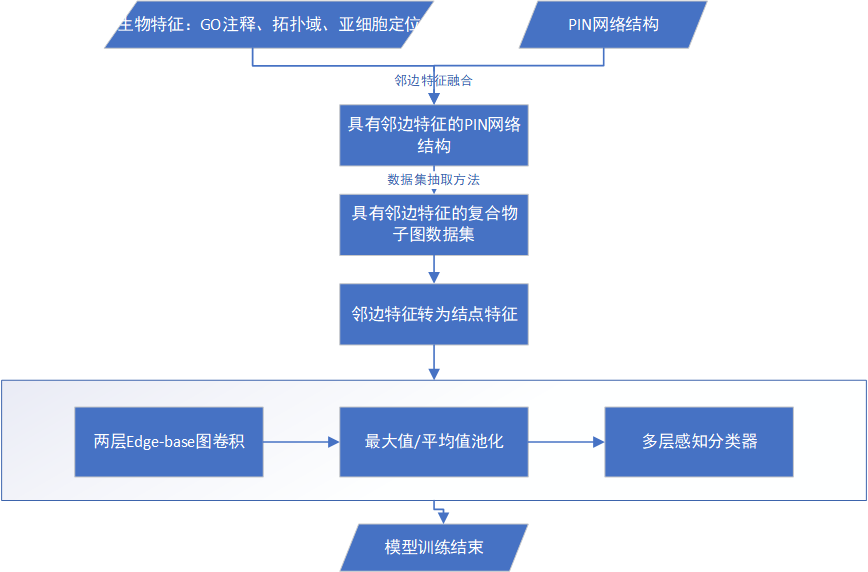
\includegraphics[width=12cm]{edge-classification-flow}
    \caption{基于生物特征的分类模型总体流程}
    \label{fig:edge-classification-flow}
\end{figure}
最终将子图的蛋白质结点特征做平均池化,作为蛋白质复合物特征的输出,以多层感知器预测复合物的分类结果。

\section{特征融合模型}
\label{section:fusionfeatBaseModel}
\subsection{模型提出}
\label{subsection:fusion:Modelget}

模型\ref{section:GlobalfeatBaseModel}和模型\ref{section:biofeatBaseModel}分别是结点嵌入和邻边嵌入模型,蛋白质复合物的形成和蛋白质以及蛋白质互作相关。
普通的GCN模型只能将邻边特征转换为结点特征之后再进行图卷积运算,这个过程将邻边特征均匀的分配给了其相邻的结点,在模型训练过程中不再将邻边作为独立的计算元素。这种情形下,邻边特征只能作为结点特征的补充,无法与复合物互作网络动态的结合起来。

为了将邻边特征与结点特征整合到模型的动态参数更新中,本节基于消息传递网络(Message Passing Neural Network,简称MPNN)提出蛋白质复合物特征融合模型,同时处理蛋白质复合物子图中的结点数据和邻边数据,将生物数据、全局拓扑特征以及局部拓扑特征动态的融合起来。

\subsection{模型细节}
\label{subsection:fusion:Modeldetail}

融合模型是基于MPNN网络的改进,MPNN网络是一种基于消息传递的图结构学习框架,不同于图卷积模型必须将特征绑定到结点,MPNN将图结构的特征当成消息,特征在结构中的流动被视为消息的传递。在此框架下,图卷积神经网络可以被当作MPNN的特例,是只传递结点消息的MPNN网络。
MPNN网络的具体实现如式\ref{equ:MPNNPassing}所示。

\begin{equation}
    \label{equ:MPNNPassing}
    m_v^{t+1} = \sum_{w \in N_{(v)}}M_t(h_v^t,h_w^t,e_{vw}^t)
\end{equation}

\begin{equation}
    \label{equ:MPNNReadout}
    h_v^{t+1} = U_t(h_v^t,m_v^{t+1})
\end{equation}
其中$N_{(v)}$表示图中结点$v$的邻居,$t$为时间步。公式\ref{equ:MPNNPassing}表示消息传递阶段(Message Passing),$M_t$表示消息传递的更新函数,代表结点w向结点v传递消息的过程中,其传递的消息$h_v^t,h_w^t,e_{vw}$的更新方式。公式\ref{equ:MPNNReadout}表示更新阶段,$U_t$表示更新阶段的函数,代表结点v汇总所有周围消息后的数据更新方式。

为了使得结点特征和邻边特征具有融合的能力,蛋白质复合物特征融合模型中采用了结点更新邻边,邻边更新结点的方式。在每一层的MPNN过程中,结点t时刻特征更新为邻边t+1时刻特征、邻边t特征更新为结点t+1时刻特征。结点特征的更新具体方法如下所示,其中$Linear$为一层感知器。
\begin{equation}
    \label{equ:MineMPNNPassing}
    m_v^{t+1} = \sum_{w \in N_{(v)}}Linear^t(e_{vw}^t)
\end{equation}

\begin{equation}
    \label{equ:MineMPNNReadout}
    h_v^{t+1} = Max(h_v^t,m_v^{t+1})
\end{equation}
从式中可以看出,结点的特征更新来源分为两部分,其一为汇聚所有邻边的特征$e_{vw}^t$,同时为了保留一部分结点中具有关键性的原始特征,其更新方式采用了MaxPooling。邻边特征的具体更新方法如下所示。
\begin{equation}
    \label{equ:MineMPNNedge}
    e_{vw}^{t+1} = Max(e_{vw}^t,Linear_0^t(m_w^{l} - m_v^{l}) + Linear_1^t m_v^{l})
\end{equation}
从式中得出,类似于结点更新模型,邻边的特征更新也可以分为两部分,最后同样采用了MaxPooling的方式保留关键邻边特征。邻边特征的更新方式综合考虑了源点到汇点的特征流动部分$m_w^{l} - m_v^{l}$以及汇点的特征保留部分$m_v^{l}$。


最后融合模型同样考虑了复合物子图的整体拓扑特征,为通过图论计算的总体拓扑结构数据,作为不可学习的特征与MPNN读出的特征拼接到一起,作为最终的图特征输出。总体拓扑特征计算参考\cite{yu_predicting_2014}。

\subsection{模型流程}
\label{subsection:fusion:Modelflow}
首先是PPI网络特征融合过程,将GO注释特征、拓扑域特征以及亚细胞定位特征嵌入到PPI网络的邻边中,将Deepwalk特征、GAE特征嵌入到PPI网络的结点中。整个PPI网络此时兼具结点和邻边特征,再在该网络的基础上按照标准集和COACH算法抽取数据集,包括标准集对应的正样本、COACH对应的中间样本和随机的负样本。
\begin{figure}[htbp]
    \centering
    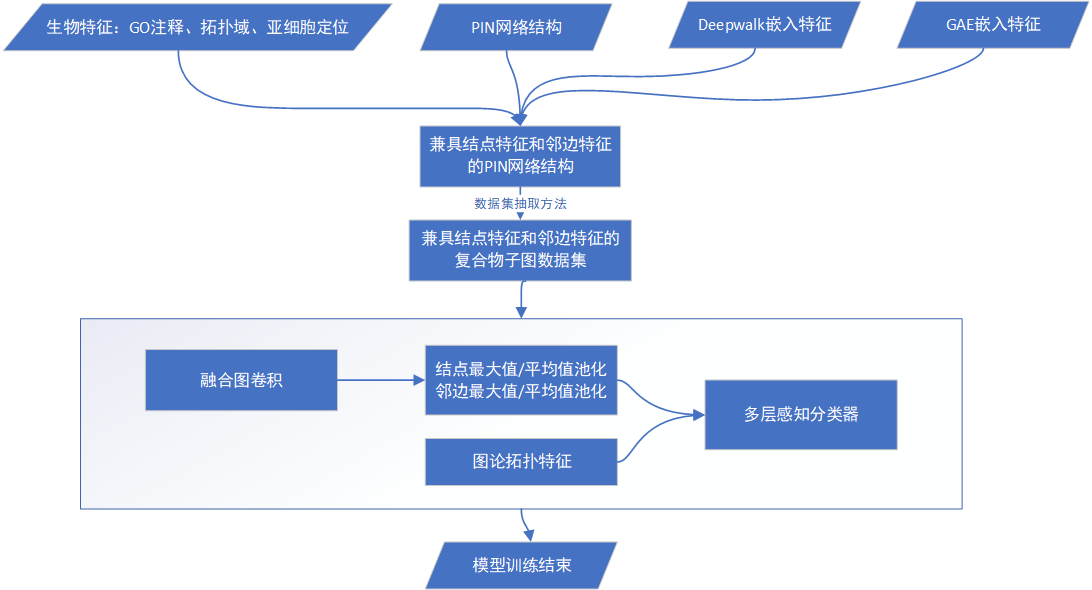
\includegraphics[width=14cm]{fusion-classification-flow}
    \caption{基于特征融合的分类模型总体流程}
    \label{fig:fusion-classification-flow}
\end{figure}

数据集中每一个样本都为蛋白质复合物子图,继承了PPI网络的结点特征和邻边特征。在所有的子图样本上训练蛋白质复合物特征融合模型,层数设置为两层。融合模型的读出阶段同时考虑如下四个方面,结点MaxPooling、结点MeanPooling、邻边MaxPooling以及邻边MeanPooling,作为子图的可学习特征。后续子图不可学习的拓扑特征和可学习特征拼接到一起,作为最终的子图特征输出。分类阶段采用了两层感知器预测分类结果和评分结果。


